\documentclass[11pt,a4paper]{article}
\usepackage[utf8]{inputenc}
\usepackage[french]{babel}
\usepackage[T1]{fontenc}

\usepackage{amsmath}
\usepackage{amsfonts}
\usepackage{amssymb}

\newcommand{\NomAuteur}{Fabrice BOISSIER}
\newcommand{\TitreMatiere}{Algorithmique 2}
\newcommand{\NomUniv}{EPITA - Bachelor Cyber Sécurité}
\newcommand{\NiveauUniv}{CYBER1}
\newcommand{\NumGroupe}{CYBER1}
\newcommand{\AnneeUniv}{2024-2025}
\newcommand{\DateExam}{juin 2025}
%\newcommand{\TypeExam}{Examen - SUJET 2}
\newcommand{\TypeExam}{Partiel (Sujet A) CORRECTION}
\newcommand{\TitreExam}{\TitreMatiere}
\newcommand{\DureeExam}{2h00}
\newcommand{\MyWaterMark}{\AnneeUniv} % Watermark de protection


% Ajout de mes classes & definitions
\usepackage{MetalExam} % Appelle un .sty

% "Tableau" et pas "Table"
\addto\captionsfrench{\def\tablename{Tableau}}

%%%%%%%%%%%%%%%%%%%%%%%
%Header
%%%%%%%%%%%%%%%%%%%%%%%
\lhead{\TypeExam}							%Gauche Haut
\chead{\NomUniv}							%Centre Haut
\rhead{\NumGroupe}							%Droite Haut
\lfoot{\DateExam}							%Gauche Bas
\cfoot{\thepage{} / \pageref*{LastPage}}	%Centre Bas
\rfoot{\texttt{\TitreMatiere}}				%Droite Bas

%%%%%

\usepackage{tabularx}

\newlength{\LabelWidth}%
%\setlength{\LabelWidth}{1.3in}%
\setlength{\LabelWidth}{1cm}%
%\settowidth{\LabelWidth}{Employee E-mail:}%  Specify the widest text here.

% Optional first parameter here specifies the alignment of
% the text within the \makebox.  Default is [l] for left
% alignment. Other options are [r] and [c] for right and center
\newcommand*{\AdjustSize}[2][l]{\makebox[\LabelWidth][#1]{#2}}%


\definecolor{mGreen}{rgb}{0,0.6,0}
\definecolor{mGray}{rgb}{0.5,0.5,0.5}
\definecolor{mPurple}{rgb}{0.58,0,0.82}
\definecolor{backgroundColour}{rgb}{0.95,0.95,0.92}

\lstdefinestyle{CStyle}{
    backgroundcolor=\color{backgroundColour},
    commentstyle=\color{mGreen},
    keywordstyle=\color{magenta},
    numberstyle=\tiny\color{mGray},
    stringstyle=\color{mPurple},
    basicstyle=\footnotesize,
    breakatwhitespace=false,
    breaklines=true,
    captionpos=b,
    keepspaces=true,
    numbers=left,
    numbersep=5pt,
    showspaces=false,
    showstringspaces=false,
    showtabs=false,
    tabsize=2,
    language=C
}


\hyphenation{op-tical net-works SIGKILL}

%%%%%%%%%%%%%%%%%%%%%%%%%%%%%%%%%%%%%%%%%%%%

% Arbre de décision :

\forestset{
  default preamble={
    before typesetting nodes={
      !r.replace by={[, coordinate, append]}
    },
    where n children=0{
      tier=word,
    }{
      diamond, aspect=2,
    },
    where level=0{}{
      if n=1{
        edge label={node[pos=.2, above] {Y}},
      }{
        edge label={node[pos=.2, above] {N}},
      }
    },
    for tree={
      edge+={thick, -Latex},
      math content,
      s sep'+=1cm,
      draw,
      thick,
      edge path'={ (!u) -| (.parent)},
    }
  }
}

%%%%%%%%%%%%%%%%%%%%%%%%%%%%%%%%%%%%%%%%%%%%

\begin{document}

%\MakeExamTitleDuree     % Pour afficher la duree
\MakeExamTitle                   % Ne pas afficher la duree

%% \MakeStudentName    %% A reutiliser sur chaque nouvelle page

\bigskip
%\bigskip

Vous devez respecter les consignes suivantes, sous peine de 0 :

\begin{table}[ht!]
  \begin{minipage}{0.45\textwidth}

\begin{enumerate}[label=\Roman*)]
\item Lisez le sujet en entier avec attention
\item Répondez sur le sujet
\item Ne trichez pas
\item Ne détachez pas les agrafes du sujet
\end{enumerate}

  \end{minipage}
  \hfillx
  \begin{minipage}{0.55\textwidth}

\begin{enumerate}[label=\Roman*),start=5]
\item \'Ecrivez lisiblement vos réponses (si nécessaire en majuscules)
%\item Vous devez écrire dans le langage algorithmique classique ou en C (donc pas de Python ou autre)
\item Vous devez écrire les algorithmes et structures en langage C (donc pas de Python ou autre)
\end{enumerate}

  \end{minipage}
\end{table}

%\begin{enumerate}[label=\Roman*)]
%\item Lisez le sujet en entier avec attention
%\item Répondez sur le sujet
%\item Ne détachez pas les agrafes du sujet
%\item \'Ecrivez lisiblement vos réponses (si nécessaire en majuscules)
%%\item Vous devez écrire dans le langage algorithmique classique ou en C (donc pas de Python ou autre)
%\item Vous devez écrire les algorithmes et structures en langage C (donc pas de Python ou autre)
%\item Ne trichez pas
%\end{enumerate}

%\bigskip

%\vfillFirst

%\vspace*{-0.5cm}
\vspace*{-0.75cm}


% Arbres Binaires
\section{Arbres Binaires (8 points)}

\subsection*{Questions (6 points) }

\subsection{Dessinez un arbre répondant aux critères imposés (2 points) }

\begin{center}
\textit{Les arbres ne doivent pas être des arbres vides}
\end{center}

\vspace{-0.5cm}

\begin{table}[ht!]
  \centering
  \begin{minipage}{0.50\textwidth}
    \centering

\subsubsection{(0,5 point) Arbre binaire complet}

\textit{(hauteur minimale : 3)}

\medskip

\begin{tikzpicture}[
  leaf/.style = {circle, forestgreen(traditional), draw=green(htmlcssgreen), very thick},
  root/.style = {circle, harvardcrimson, draw=red, very thick},
  internal/.style = {circle, auburn, draw=auburn, very thick},
  level/.style = {sibling distance = 55mm/#1},
  level 1/.style = {sibling distance = 38mm},
  level 2/.style = {sibling distance = 19mm},
  level 3/.style = {sibling distance = 9mm},
  every node/.style = {minimum width = 2em, draw, circle},
  ]
  \node {42}
  child { node {21}
          child { node {8}
                  child { node {2} }
                  child { node {16} }
                }
          child { node {24}
                  child { node {22} }
                  child { node {32} }
                }
         }
  child { node {64}
          child { node {48}
                  child { node {46} }
                  child { node {56} }
                }
          child { node {96}
                  child { node {72} }
                  child { node {98} }
                }
        };
\end{tikzpicture}

  \end{minipage}
  \hfillx
  \begin{minipage}{0.50\textwidth}
    \centering

\subsubsection{(0,5 point) Arbre filiforme}

\textit{(hauteur minimale : 3)}

\medskip

\begin{tikzpicture}[
  leaf/.style = {circle, forestgreen(traditional), draw=green(htmlcssgreen), very thick},
  root/.style = {circle, harvardcrimson, draw=red, very thick},
  internal/.style = {circle, auburn, draw=auburn, very thick},
  level/.style = {sibling distance = 55mm/#1},
  level 1/.style = {sibling distance = 38mm},
  level 2/.style = {sibling distance = 19mm},
  level 3/.style = {sibling distance = 9mm},
  every node/.style = {minimum width = 2em, draw, circle},
  ]
  \node {42}
  child { edge from parent[draw = none] }
  child { node {64}
          child { edge from parent[draw = none] }
          child { node {96}
                  child { edge from parent[draw = none] }
                  child { node {98} }
                }
        };
\end{tikzpicture}

  \end{minipage}
\end{table}

%%%%%%%%%%%%%%%%
\vspace*{-0.5cm}
\rule{1.0\linewidth}{0.75pt}
%%%%%%%%%%%%%%%%

\begin{table}[ht!]
  \centering
  \begin{minipage}{0.50\textwidth}
    \centering

\subsubsection{(0,5 point) Arbre binaire presque complet et localement complet}

\textit{(hauteur minimale : 0)}

\medskip

\vspace*{2cm}

\begin{tikzpicture}[
  leaf/.style = {circle, forestgreen(traditional), draw=green(htmlcssgreen), very thick},
  root/.style = {circle, harvardcrimson, draw=red, very thick},
  internal/.style = {circle, auburn, draw=auburn, very thick},
  level/.style = {sibling distance = 55mm/#1},
  level 1/.style = {sibling distance = 38mm},
  level 2/.style = {sibling distance = 19mm},
  level 3/.style = {sibling distance = 9mm},
  every node/.style = {minimum width = 2em, draw, circle},
  ]
  \node {42} ;
\end{tikzpicture}

  \end{minipage}
  \hfillx
  \begin{minipage}{0.50\textwidth}
    \centering

\subsubsection{(0,5 point) Arbre binaire parfait}

\textit{(hauteur minimale : 3)}

\medskip

\begin{tikzpicture}[
  leaf/.style = {circle, forestgreen(traditional), draw=green(htmlcssgreen), very thick},
  root/.style = {circle, harvardcrimson, draw=red, very thick},
  internal/.style = {circle, auburn, draw=auburn, very thick},
  level/.style = {sibling distance = 55mm/#1},
  level 1/.style = {sibling distance = 38mm},
  level 2/.style = {sibling distance = 19mm},
  level 3/.style = {sibling distance = 9mm},
  every node/.style = {minimum width = 2em, draw, circle},
  ]
  \node {42}
  child { node {21}
          child { node {8}
                  child { node {2} }
                  child { node {16} }
                }
          child { node {24}
                  child { node {22} }
                  child { node {32} }
                }
         }
  child { node {64}
          child { node {48}
                  child { node {46} }
                  child { node {56} }
                }
          child { node {96}
                  child { node {72} }
                  child { node {98} }
                }
        };
\end{tikzpicture}

  \end{minipage}
\end{table}

\clearpage

%%%%%%%%%%%%%%%%%%%%%%%%%%%%%%%%%%%%%%%%%%%%%%%

\subsection{Répondez aux différentes questions concernant l'arbre suivant (4 points) }

\bigskip

% lvl1 = 55mm, lvl2 = 30mm, lvl3 = 15mm, lvl4 = 10mm
\begin{center}
\begin{tikzpicture}[sibling distance=1.5cm,
  level/.style = {sibling distance = 55mm/#1},
  level 1/.style = {sibling distance = 70mm},
  level 2/.style = {sibling distance = 35mm},
  level 3/.style = {sibling distance = 18mm},
  level 4/.style = {sibling distance = 8mm},
  every node/.style = {minimum width = 2em, draw, circle},
  ]
  \node (n1E) {E}
  child { node (n2N) {N}
          child { node (n3T) {T}
                  child { node (n4S) {S}
                          child { node (n5R) {R} }
                          child { node (n6E) {E} }
                        }
                  child { node (n7C) {C}
                          child { node (n8P) {P} }
                          child { node (n9E) {E} }
                        }
                }
          child { node (n10O) {O}
                  child { node (n11Z) {Z}
                          child { node (n12E) {E} }
                          child { node [draw=none] (nX) {\phantom{X}} edge from parent [draw=none] }
                        }
                  child { node (n13M) {M} }
                }
         }
   child { node (n14T) {T}
           child { node (n15T) {T}
                   child { node (n16A) {A} }
                   child { node (n17U) {U} }
                 }
           child { node (n18I) {I}
                   child { node (n19O) {O} }
                   child { node (n20R) {R}
                           child { node [draw=none] (nX) {\phantom{X}} edge from parent [draw=none] }
                           child { node [draw=none] (nX) {\phantom{X}} edge from parent [draw=none] }
                         }
                 }
        };
\end{tikzpicture}
%  child { node [draw=none] (nX) {\phantom{X}} edge from parent [draw=none] }
\end{center}


\subsubsection{(1,5 point) Indiquez toutes les propriétés que possède cet arbre : }

\bigskip

\begin{tabular}{L{2cm}C{1.5cm} L{2cm}C{1.5cm} L{2cm}C{1.5cm} L{2.5cm}C{1.5cm}}
Arité : 2 & & Taille : 20 & & Hauteur : 4 & & Nb feuilles : 10 & \\
\end{tabular}

\medskip

\begin{table}[ht!]
  \centering
  \begin{minipage}{0.50\textwidth}
    \centering

\begin{itemize}
  \item[\CaseCoche] Arbre binaire strict / localement complet \phantom{()}
  \item[\CaseCoche] Arbre binaire parfait \phantom{()}
  \item[\CaseCoche] Peigne gauche \phantom{()}
\end{itemize}

  \end{minipage}
  \hfillx
  \begin{minipage}{0.50\textwidth}
    \centering

\begin{itemize}
  \item[\checkmark] Arbre binaire (presque) complet \phantom{()}
%  \item[\CaseCoche] Arbre binaire (presque) complet \phantom{()}
  \item[\CaseCoche] Arbre filiforme \phantom{()}
  \item[\CaseCoche] Peigne droit \phantom{()}
\end{itemize}

  \end{minipage}
\end{table}


%\bigskip

\subsubsection{(2 points) \'Ecrivez les clés lors d'un parcours profondeur main gauche de l'arbre dans les 3 ordres ainsi que lors d'un parcours largeur : }

%\medskip

Parcours profondeur :

\medskip

\centerline{
%\begin{tabular}{L{2.5cm} C{0.5cm}C{0.5cm}C{0.5cm}C{0.5cm}C{0.5cm} C{0.5cm}C{0.5cm}C{0.5cm}C{0.5cm} C{0.5cm}C{0.5cm}C{0.5cm}C{0.5cm} C{0.5cm}C{0.5cm}C{0.5cm} C{0.5cm}C{0.5cm}C{0.5cm}}
\begin{tabular}{L{2.5cm} C{0.35cm}C{0.35cm}C{0.35cm}C{0.35cm}C{0.35cm} C{0.35cm}C{0.35cm}C{0.35cm}C{0.35cm} C{0.35cm}C{0.35cm}C{0.35cm}C{0.35cm} C{0.3cm}C{0.35cm}C{0.35cm} C{0.35cm}C{0.35cm}C{0.35cm} C{0.35cm}}
 & & & & & & & & & & & & & & & & & & & \\
ordre préfixe : & E & N & T & S & R & E & C & P & E & O & Z & E & M & T & T & A & U & I & O & R \\
 & & & & & & & & & & & & & & & & & & & \\
ordre infixe :  & R & S & E & T & P & C & E & N & E & Z & O & M & E & A & T & U & T & O & I & R \\
 & & & & & & & & & & & & & & & & & & & \\
ordre suffixe : & R & E & S & P & E & C & T & E & Z & M & O & N & A & U & T & O & R & I & T & E \\
\end{tabular}
}

%\bigskip
\vspace*{0.75cm}

Parcours largeur :

\medskip

\centerline{
%\begin{tabular}{L{2.5cm} C{0.5cm}C{0.5cm}C{0.5cm}C{0.5cm}C{0.5cm} C{0.5cm}C{0.5cm}C{0.5cm}C{0.5cm} C{0.5cm}C{0.5cm}C{0.5cm}C{0.5cm} C{0.5cm}C{0.5cm}C{0.5cm} C{0.5cm}C{0.5cm}C{0.5cm}}
\begin{tabular}{L{2.5cm} C{0.35cm}C{0.35cm}C{0.35cm}C{0.35cm}C{0.35cm} C{0.35cm}C{0.35cm}C{0.35cm}C{0.35cm} C{0.35cm}C{0.35cm}C{0.35cm}C{0.35cm} C{0.3cm}C{0.35cm}C{0.35cm} C{0.35cm}C{0.35cm}C{0.35cm} C{0.35cm}}
 & & & & & & & & & & & & & & & & & & & \\
ordre :  & E & N & T & T & O & T & I & S & C & Z & M & A & U & O & R & R & E & P & E & E \\
\end{tabular}
}

\medskip

\subsubsection{(0,5 point) Indiquez la profondeur et le numéro hiérarchique des nœuds suivants : }

\medskip

\centerline{
\begin{tabular}{ | C{1cm}|C{1.75cm}|C{2.65cm} |   p{2.0cm}   | C{1cm}|C{1.75cm}|C{2.65cm} | }
\cline{1-3}\cline{5-7}
 & Profondeur & N\textsuperscript{o} hiérarchique &
 &
 & Profondeur & N\textsuperscript{o} hiérarchique \\
\cline{1-3}\cline{5-7}
\multirow{3}{*}{Z} & \multirow{3}{*}{3} & \multirow{3}{*}{10} &
 &
\multirow{3}{*}{P} & \multirow{3}{*}{4} & \multirow{3}{*}{18} \\
 & & & & & & \\
 & & & & & & \\
\cline{1-3}\cline{5-7}
\end{tabular}
}

\clearpage

%%%%%%%%%%%%%%%%%%%%%%%%%%%%%%%%%%%%%%%%%%%%%%%

\subsection*{Algorithmes (2 points) }

\subsection{(1 point) \'Ecrivez une procédure \og \textit{BFS} \fg{} effectuant un parcours largeur dans un arbre binaire, et affichant les nœuds (l'arbre est de type \textit{node*}) : }

\begin{center}
\GrilleReponseN{12}
\end{center}

%%%%%%%%%%%%%%%%%%%%%%%%%%%%%%%%%%%%%%%%%%%%%%%

\subsection{(1 point) \'Ecrivez une procédure \og \textit{DFS} \fg{} effectuant un parcours profondeur main gauche dans un arbre binaire, et affichant les nœuds dans les 3 ordres (l'arbre est de type \textit{node*}) : }

\begin{center}
\GrilleReponseN{9}
\end{center}


\clearpage

%%%%%%%%%%%%%%%%%%%%%%%%%%%%%%%%%%%%%%%%%%%%%%%%%%%%%%%%%%%%%%%%%
%%%%%%%%%%%%%%%%%%%%%%%%%%%%%%%%%%%%%%%%%%%%%%%%%%%%%%%%%%%%%%%%%
%%%%%%%%%%%%%%%%%%%%%%%%%%%%%%%%%%%%%%%%%%%%%%%%%%%%%%%%%%%%%%%%%

% Arbres Binaires de Recherche
\section{Arbres Binaires de Recherche (8 points)}

\subsection*{Questions (4 points) }

\subsection{(4 points) Dessinez le résultat des opérations successives : }

\begin{itemize}
\item \textit{InsertLeaf(node *R, int val)} insère l'élément \og \textit{val} \fg{} en feuille dans l'ABR \og \textit{R} \fg{}
\item \textit{InsertRoot(node *R, int vat)} insère l'élément \og \textit{val} \fg{} en racine dans l'ABR \og \textit{R} \fg{}
\item \textit{RemoveFromBST(node *R, int val)} supprime l'élément \og \textit{val} \fg{} de l'ABR \og \textit{R} \fg{}
\end{itemize}

\vspace*{-0.5cm}

\begin{center}

%\'Eléments insérés : 18 - 46 - 55 - 36 - 12 - 38 - 96 - 71
%\'Eléments insérés : 46 - 18 - 55 - 36 - 12 - 38 - 96 - 71
%\'Eléments insérés : 32 - 24 - 18 - 30 - 31 - 42 - 36 - 50
%\'Eléments insérés : 32 - 24 - 18 - 30 - 31 - 42 - 36

% 1-2-3 : 42, 24, 64

\begin{table}[ht!]
  \centering
  \begin{minipage}{0.33\textwidth}
    \centering

\textit{\'Etape 1}

R = InsertLeaf(NULL, 42)

\medskip

\vspace*{1cm}

\begin{tikzpicture}[
  leaf/.style = {circle, forestgreen(traditional), draw=green(htmlcssgreen), very thick},
  root/.style = {circle, harvardcrimson, draw=red, very thick},
  internal/.style = {circle, auburn, draw=auburn, very thick},
  level/.style = {sibling distance = 55mm/#1},
  level 1/.style = {sibling distance = 38mm},
  level 2/.style = {sibling distance = 19mm},
  level 3/.style = {sibling distance = 9mm},
  every node/.style = {minimum width = 2em, draw, circle},
  ]
  \node {42};
\end{tikzpicture}

\vspace*{1cm}

  \end{minipage}
  \hfillx
  \begin{minipage}{0.33\textwidth}
    \centering

\textit{\'Etape 2}

R = InsertLeaf(R, 24)

\medskip

\begin{tikzpicture}[
  level 1/.style = {sibling distance = 20mm},
  every node/.style = {minimum width = 2em, draw, circle},
  ]
  \node {42}
  child { node {24} }
  child { edge from parent[draw = none]
        };
\end{tikzpicture}

\vspace*{0.5cm}

  \end{minipage}
  \hfillx
  \begin{minipage}{0.33\textwidth}
    \centering

\textit{\'Etape 3}

R = InsertLeaf(R, 64)

\medskip

\begin{tikzpicture}[
  level 1/.style = {sibling distance = 20mm},
  every node/.style = {minimum width = 2em, draw, circle},
  ]
  \node {42}
  child { node {24} }
  child { node {64}
        };
\end{tikzpicture}

\vspace*{0.5cm}

  \end{minipage}
\end{table}

%%%%%%%%%%%%%%%%
\vspace*{-0.5cm}
\rule{1.0\linewidth}{0.75pt}
%%%%%%%%%%%%%%%%


% 4-5-6 : 32, 56, 36

\begin{table}[ht!]
  \centering
  \begin{minipage}{0.33\textwidth}
    \centering

\textit{\'Etape 4}

R = InsertLeaf(R, 32)

\medskip

\begin{tikzpicture}[
  level 1/.style = {sibling distance = 25mm},
  level 2/.style = {sibling distance = 15mm},
  every node/.style = {minimum width = 2em, draw, circle},
  ]
  \node {42}
  child { node {24}
          child { edge from parent[draw = none] }
          child { node {32} }
        }
  child { node {64}
        };
\end{tikzpicture}

\vspace*{2cm}

  \end{minipage}
  \hfillx
  \begin{minipage}{0.33\textwidth}
    \centering

\textit{\'Etape 5}

R = InsertLeaf(R, 56)

\medskip

\begin{tikzpicture}[
  level 1/.style = {sibling distance = 25mm},
  level 2/.style = {sibling distance = 15mm},
  every node/.style = {minimum width = 2em, draw, circle},
  ]
  \node {42}
  child { node {24}
          child { edge from parent[draw = none] }
          child { node {32} }
        }
  child { node {64}
          child { node {56} }
          child { edge from parent[draw = none] }
        };
\end{tikzpicture}

\vspace*{2cm}

  \end{minipage}
  \hfillx
  \begin{minipage}{0.33\textwidth}
    \centering

\textit{\'Etape 6}

R = InsertLeaf(R, 36)

\medskip

\begin{tikzpicture}[
  level 1/.style = {sibling distance = 30mm},
  level 2/.style = {sibling distance = 15mm},
  level 3/.style = {sibling distance = 9mm},
  every node/.style = {minimum width = 2em, draw, circle},
  ]
  \node {42}
  child { node {24}
          child { edge from parent[draw = none] }
          child { node {32}
                  child { edge from parent[draw = none] }
                  child { node {36} }
                }
        }
  child { node {64}
          child { node {56} }
          child { edge from parent[draw = none] }
        };
\end{tikzpicture}

\vspace*{0.5cm}

  \end{minipage}
\end{table}

%%%%%%%%%%%%%%%%
\vspace*{-0.5cm}
\rule{1.0\linewidth}{0.75pt}
%%%%%%%%%%%%%%%%


% 7-8 : R34, 72

\begin{table}[ht!]
  \centering
  \begin{minipage}{0.50\textwidth}
    \centering

\textit{\'Etape 7}

R = \textit{InsertRoot}(R, 34)

\medskip

\begin{tikzpicture}[
  level 1/.style = {sibling distance = 30mm},
  level 2/.style = {sibling distance = 15mm},
  level 3/.style = {sibling distance = 9mm},
  every node/.style = {minimum width = 2em, draw, circle},
  ]
  \node {34}
  child { node {24}
          child { edge from parent[draw = none] }
          child { node {32} }
        }
  child { node {42}
          child { node {36} }
          child { node {64}
                  child { node {56} }
                  child { edge from parent[draw = none] }
                }
        };
\end{tikzpicture}

  \end{minipage}
  \hfillx
  \begin{minipage}{0.50\textwidth}
    \centering

\textit{\'Etape 8}

R = InsertLeaf(R, 72)

\medskip

\begin{tikzpicture}[
  level 1/.style = {sibling distance = 30mm},
  level 2/.style = {sibling distance = 15mm},
  level 3/.style = {sibling distance = 9mm},
  every node/.style = {minimum width = 2em, draw, circle},
  ]
  \node {34}
  child { node {24}
          child { edge from parent[draw = none] }
          child { node {32} }
        }
  child { node {42}
          child { node {36} }
          child { node {64}
                  child { node {56} }
                  child { node {72} }
                }
        };
\end{tikzpicture}

  \end{minipage}
\end{table}

%%%%%%%%%%
\clearpage
%%%%%%%%%%

% 9-10 : R38, -42

\begin{table}[ht!]
  \centering
  \begin{minipage}{0.50\textwidth}
    \centering

\textit{\'Etape 9}

R = \textit{InsertRoot}(R, 38)

\medskip

\begin{tikzpicture}[
  level 1/.style = {sibling distance = 30mm},
  level 2/.style = {sibling distance = 15mm},
  level 3/.style = {sibling distance = 9mm},
  every node/.style = {minimum width = 2em, draw, circle},
  ]
  \node {38}
  child { node {34}
          child { node {24}
                  child { edge from parent[draw = none] }
                  child { node {32} }
                }
          child { node {36} }
        }
  child { node {42}
          child { edge from parent[draw = none] }
          child { node {64}
                  child { node {56} }
                  child { node {72} }
                }
        };
\end{tikzpicture}

\vspace*{0.5cm}

  \end{minipage}
  \hfillx
  \begin{minipage}{0.50\textwidth}
    \centering

\textit{\'Etape 10}

R = RemoveFromBST(R, 42)

\medskip

\begin{tikzpicture}[
  level 1/.style = {sibling distance = 30mm},
  level 2/.style = {sibling distance = 15mm},
  level 3/.style = {sibling distance = 9mm},
  every node/.style = {minimum width = 2em, draw, circle},
  ]
  \node {38}
  child { node {34}
          child { node {24}
                  child { edge from parent[draw = none] }
                  child { node {32} }
                }
          child { node {36} }
        }
  child { node {64}
          child { node {56} }
          child { node {72} }
        };
\end{tikzpicture}

\vspace*{0.5cm}

  \end{minipage}
\end{table}

%%%%%%%%%%%%%%%%
\vspace*{-0.5cm}
\rule{1.0\linewidth}{0.75pt}
%%%%%%%%%%%%%%%%


% 9-10 : -38, R60

\begin{table}[ht!]
  \centering
  \begin{minipage}{0.50\textwidth}
    \centering

\textit{\'Etape 11}

R = RemoveFromBST(R, 38)

\medskip

\begin{tikzpicture}[
  level 1/.style = {sibling distance = 30mm},
  level 2/.style = {sibling distance = 15mm},
  level 3/.style = {sibling distance = 9mm},
  every node/.style = {minimum width = 2em, draw, circle},
  ]
  \node {36}
  child { node {34}
          child { node {24}
                  child { edge from parent[draw = none] }
                  child { node {32} }
                }
          child { edge from parent[draw = none] }
        }
  child { node {64}
          child { node {56} }
          child { node {72} }
        };
\end{tikzpicture}

\vspace*{1cm}

  \end{minipage}
  \hfillx
  \begin{minipage}{0.50\textwidth}
    \centering

\textit{\'Etape 12}

R = \textit{InsertRoot}(R, 60)

\medskip

\begin{tikzpicture}[
  level 1/.style = {sibling distance = 30mm},
  level 2/.style = {sibling distance = 15mm},
  level 3/.style = {sibling distance = 9mm},
  every node/.style = {minimum width = 2em, draw, circle},
  ]
  \node {60}
  child { node {36}
          child { node {34}
                  child { node {24}
                          child { edge from parent[draw = none] }
                          child { node {32} }
                        }
                  child { edge from parent[draw = none] }
                }
          child { node {56} }
        }
  child { node {64}
          child { edge from parent[draw = none] }
          child { node {72} }
        };
\end{tikzpicture}

  \end{minipage}
\end{table}

%%%%%%%%%%%%%%%%
\vspace*{-0.5cm}
\rule{1.0\linewidth}{0.75pt}
%%%%%%%%%%%%%%%%

%Indiquez combien de rotations droite gauche et gauche droite ont été effectuées dans l'insertion en AVL des précédents éléments (1 point) :
%
%\begin{table}[ht!]
%  \centering
%  \begin{minipage}{0.50\textwidth}
%
%RDG :
%
%  \end{minipage}
%  \hfillx
%  \begin{minipage}{0.50\textwidth}
%
%RGD :
%
%  \end{minipage}
%\end{table}

\end{center}

\textit{(Espace libre pour dessiner) - Attention : il reste encore des exercices après !}

\vspace*{-0.25cm}

\begin{center}
{\small \textit{(ces dessins ne sont pas de moi)}}

\begin{table}[ht!]
  \centering
  \begin{minipage}{0.50\textwidth}
    \centering

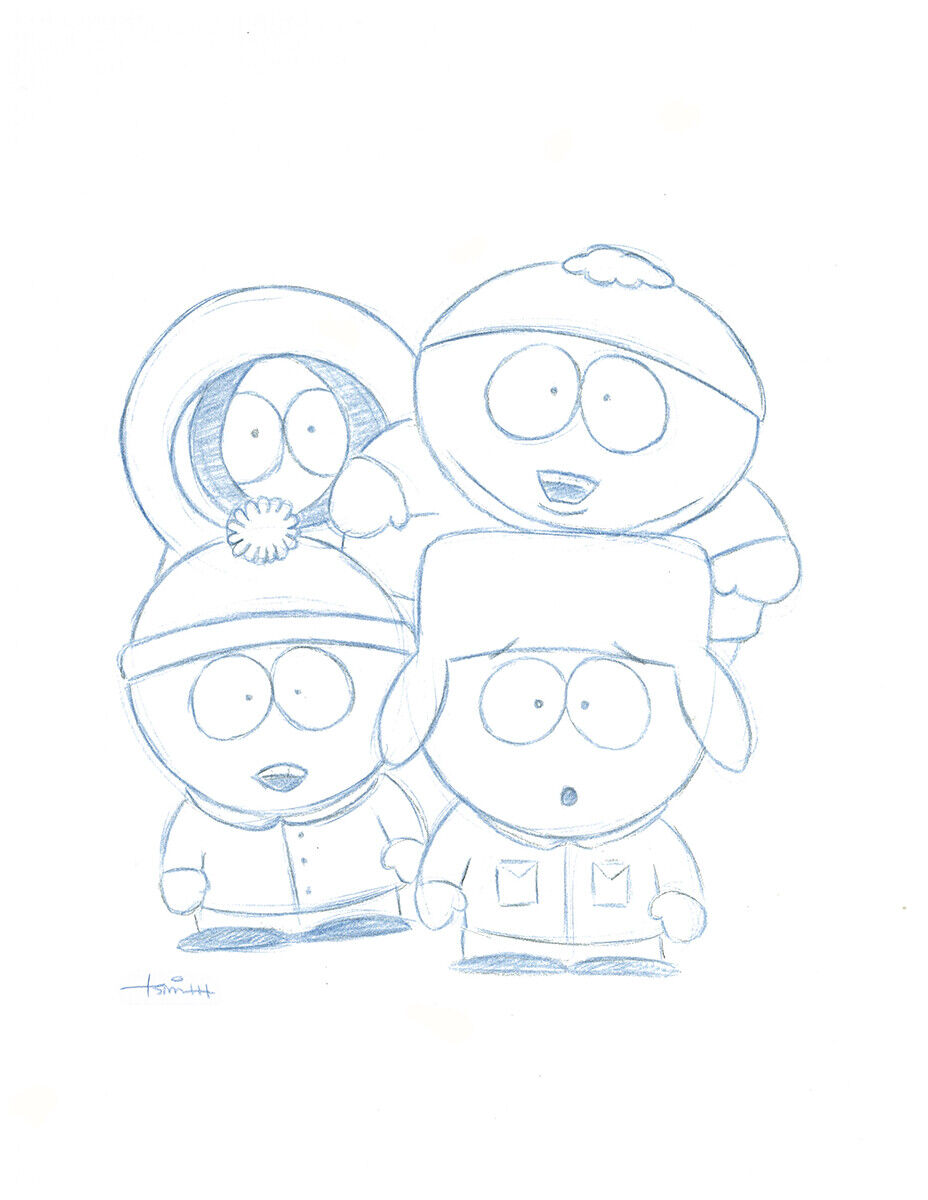
\includegraphics[trim={1.5cm 3cm 2cm 4cm},clip,scale=0.55]{img/sp_1.jpg}

  \end{minipage}
  \hfillx
  \begin{minipage}{0.50\textwidth}
    \centering

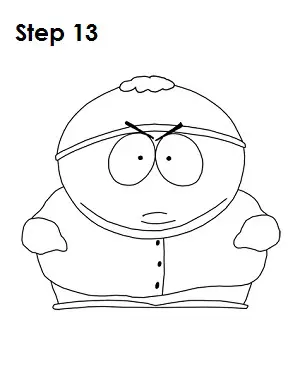
\includegraphics[trim={0.5cm 2cm 0.5cm 2cm},clip,scale=0.55]{img/sp_2.png}

   \end{minipage}
\end{table}

\end{center}

\clearpage

%%%%%%%%%%%%%%%%%%%%%%%%%%%%%%%%%%%%%%%%%%%%%%%%%%%%%%%%

\subsection*{Algorithmes (4 points) }

\subsection{(2 points) \'Ecrivez une fonction \textit{BSTSearch} recherchant un entier dans un arbre binaire de recherche et renvoyant l'adresse de son nœud. Si l'élément n'est pas trouvé, la fonction doit renvoyer \TTBF{NULL} : }

\begin{center}
\GrilleReponseN{8}
\end{center}

%%%%%%%%%%%%%%%%%%%%%%%%%%%%%%%%%%%%%%%

\subsection{(2 points) \'Ecrivez une fonction \textit{InsertLeaf} ajoutant en feuille un élément dans un arbre binaire de recherche : }

\begin{center}
\GrilleReponseN{13}
\end{center}

\clearpage

%%%%%%%%%%%%%%%%%%%%%%%%%%%%%%%%%%%%%%%%%%%%%%%%%%%%%%%%%%%%%%%%%
%%%%%%%%%%%%%%%%%%%%%%%%%%%%%%%%%%%%%%%%%%%%%%%%%%%%%%%%%%%%%%%%%
%%%%%%%%%%%%%%%%%%%%%%%%%%%%%%%%%%%%%%%%%%%%%%%%%%%%%%%%%%%%%%%%%

\vfillFirst

\begin{center}
{\LARGE \textbf{Problème} }
\end{center}

\vfillLast

\clearpage

%%%%%%%%%%%%%%%%%%%%%%%%%%%%%%%%%%%%%%%%%%%%%%%%%%%%%%%%%%%%%%%%%

\vfillFirst

% Problème
\section{Arbres de Décision (4 points) }

%\subsection*{Arbres de Décision}

\noindent Dans le monde de l'intelligence artificielle, il existe de très (trop) nombreux sous-domaines, dont le \textit{décisionnel} ou \textit{aide à la décision} impliquant d'analyser des données pour orienter les décisions, voire, permettre une prise de décision automatique.
Parmi les nombreuses méthodes proposées dans la science des données, l'une se prénomme \textit{arbre de décisions}.
Comme leur nom le laisse entendre : il s'agit d'arbres, mais leur spécificité réside dans le fait qu'ils représentent les données analysées et permettent d'en déduire une décision.

\bigskip

\begin{center}
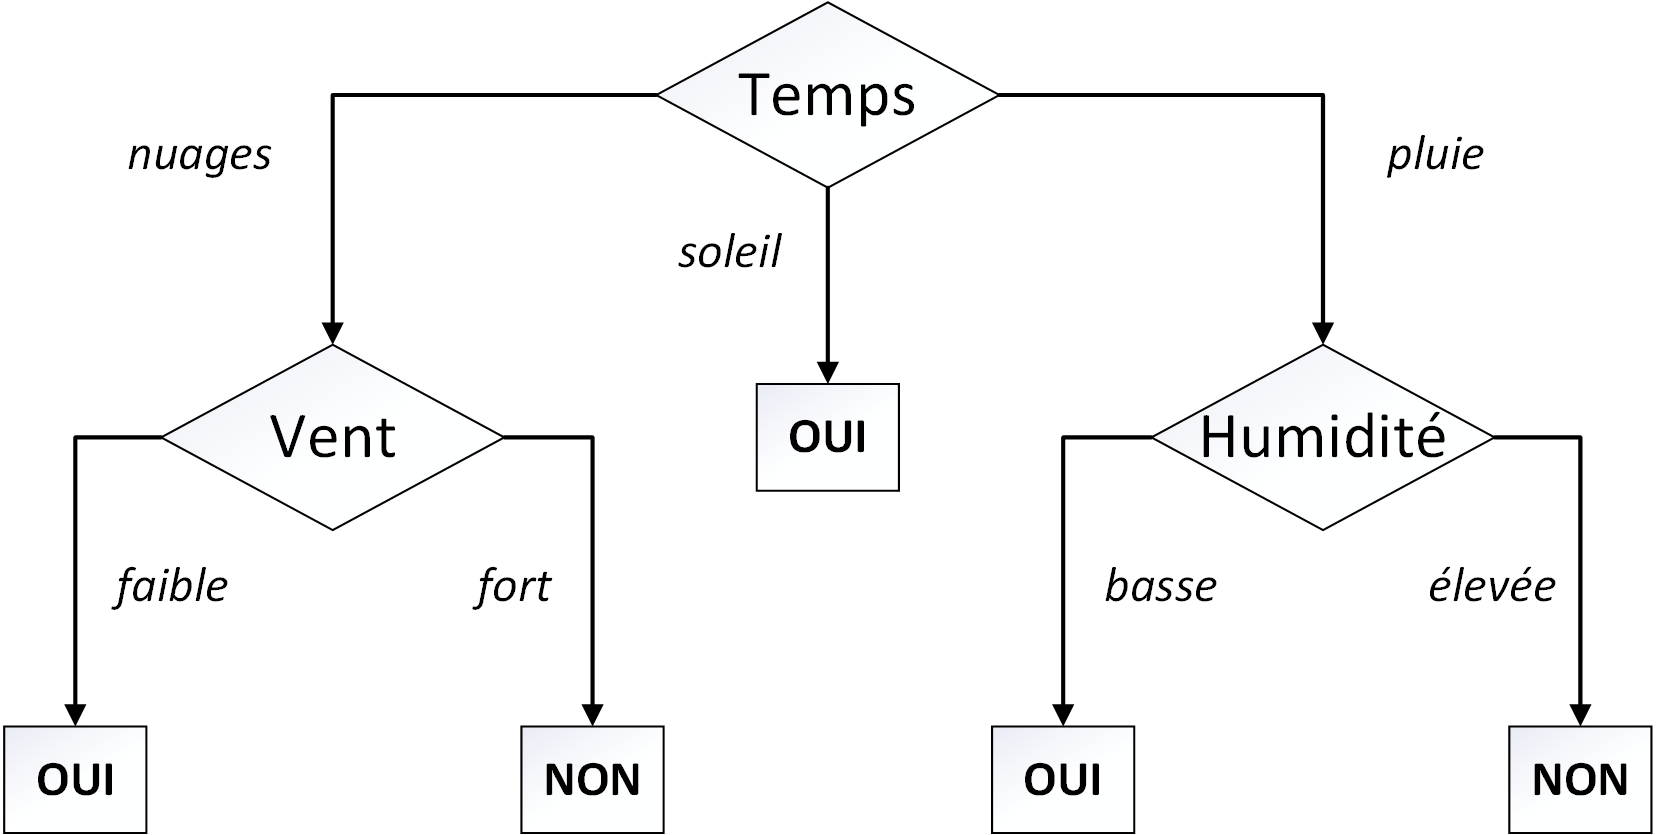
\includegraphics[scale=0.70]{img/DecisionTree_Tennis_example.png}
\end{center}

\bigskip

\noindent L'exemple le plus célèbre concerne la décision d'aller jouer (ou non) au tennis selon la météo.
Dans l'exemple précédent, si le temps est \textit{nuages} et la vitesse du vent est \textit{faible}, ou plus simplement s'il fait \textit{soleil}, alors on sortira jouer au tennis.
À l'inverse, si le temps est \textit{pluie}, avec une humidité \textit{élevée}, alors on préfèrera une autre activité.

\medskip

\noindent Les arbres de décisions sont des arbres dits \textit{généraux}, car leur arité n'est pas nécessairement binaire.
Dans le problème que vous traiterez, les arbres seront néanmoins binaires pour vous permettre d'écrire les algorithmes.

\vfillLast

\clearpage

%%%%%%%%%%%%%%%%%%%%%%%%%%%%%%%%%%%%%%%

\subsection*{[S01E08] Damien}

\noindent L'anniversaire d'\'Eric Cartman approche à grands pas, mais, le pauvre Kenny McCormick vient d'être transformé en ornithorynque par Damien (le nouveau de la classe) !
\'Eric souhaitant à tout prix obtenir sa collection de jouets MegaMan, il décide de consulter la liste des cadeaux qu'il a exigés à ses \og amis \fg{} afin de changer leur ordre (un ornithorynque ne pouvant \textit{contracter}, il ne peut donc ni effectuer d'achat au magasin de jouets ni payer de TVA à l'\'Etat).

\noindent Votre travail consiste donc à devoir (malheureusement) aider le jeune \'Eric Cartman à changer l'assignation des cadeaux de ses \og amis \fg{} en analysant l'arbre de décision suivant :

\begin{center}
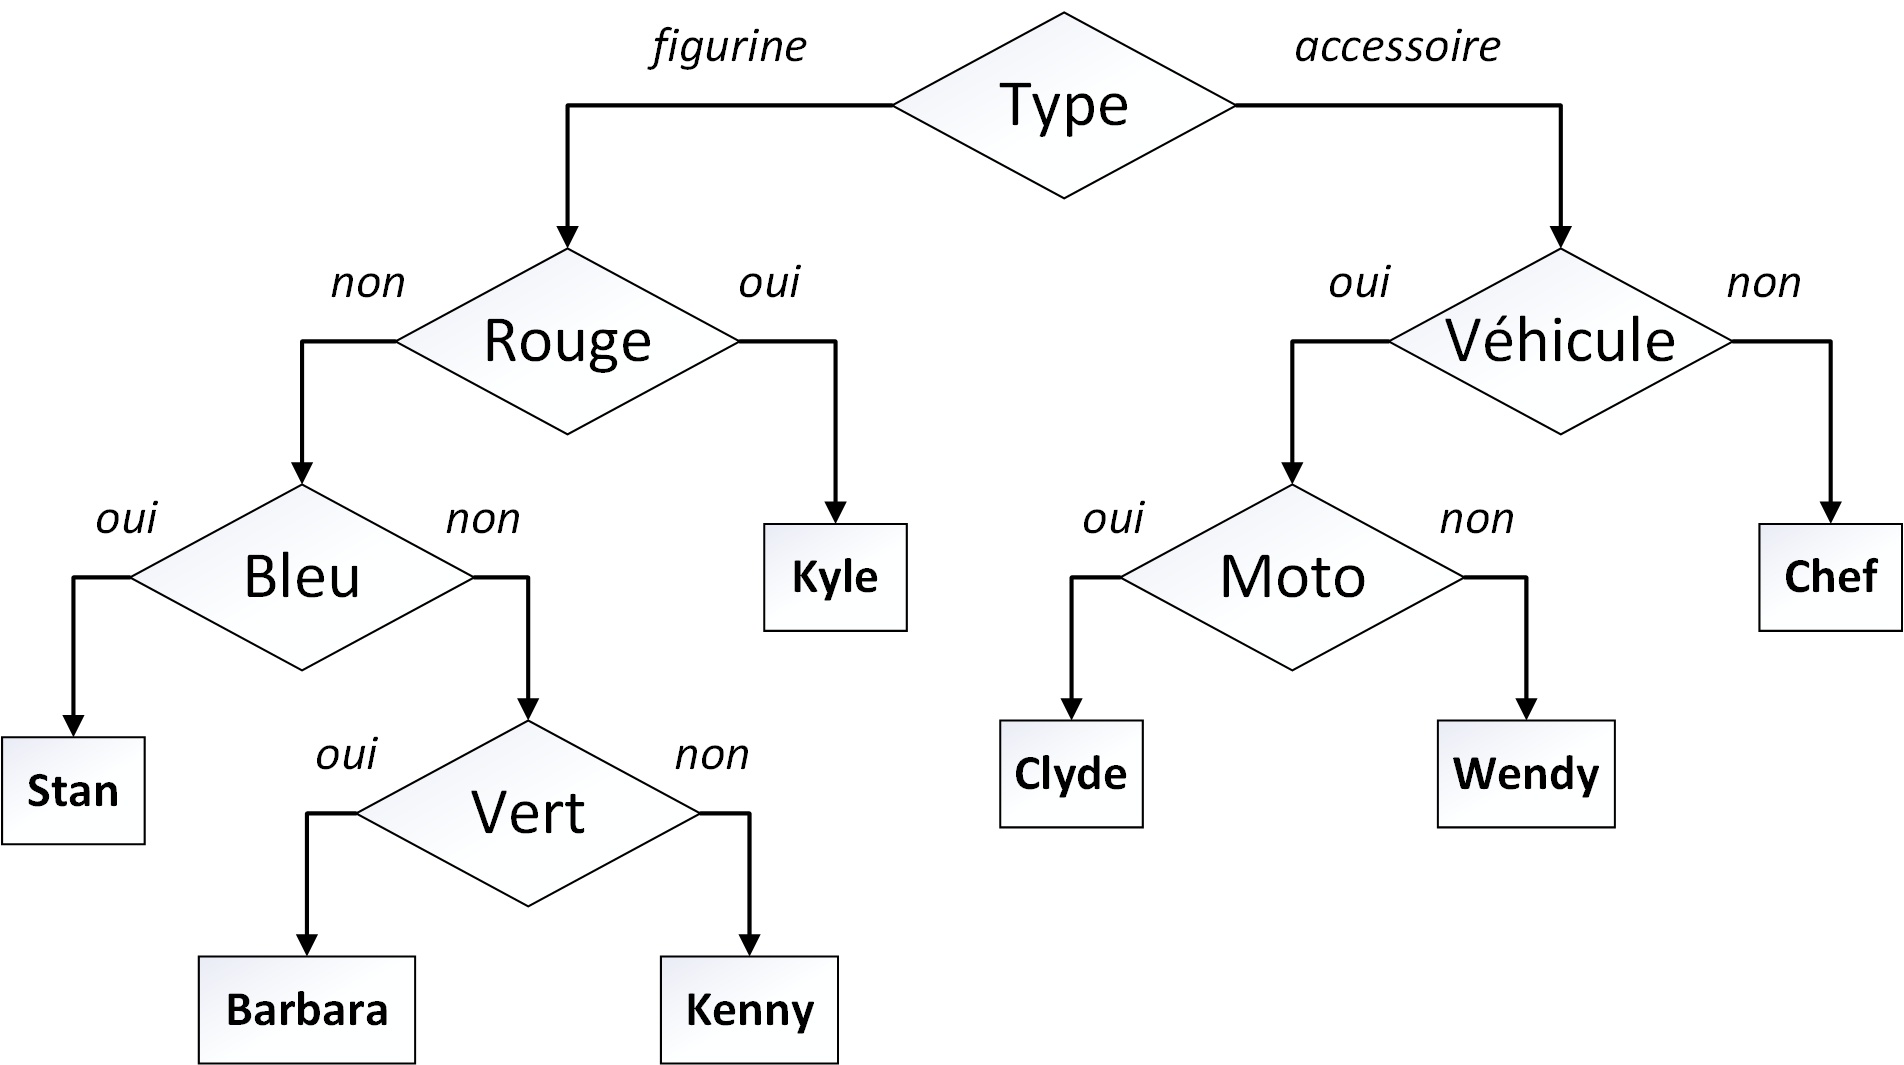
\includegraphics[scale=0.60]{img/DecisionTree_Cartman_MegaMan.png}
\end{center}

%\bigskip
%\clearpage

\subsection{(2 points) Lecture d'un arbre de décision}

%\noindent À partir de l'arbre de décision précédent et du tableau de caractéristiques suivant, indiquez qui doit apporter quel cadeau.
\noindent Indiquez qui doit apporter quel cadeau à partir de l'arbre de décision précédent.

%\medskip

\begin{center}

%\begin{tabular}{ | L{3.5cm} | c | }
%%\begin{tabular}{ | L{5cm} | C{3.5cm} | }
\begin{tabular}{ | L{3.5cm} | C{3.5cm} | C{8cm} | }
\hline
  \multirow[c]{1}{*}[0in]{\begin{minipage}{3.5cm} \centering \textbf{Jouet} \end{minipage}} &
  \textbf{Caractéristiques} &
  \textbf{Ami(e) qui doit l'apporter} \\
\hline
  \multirow[c]{3}{*}[0in]{\begin{minipage}{3.5cm} MegaMan Rouge \end{minipage}} &
  \multirow[c]{3}{*}[0in]{\begin{minipage}{3.5cm} \centering \textit{figurine}, \textit{rouge} \end{minipage}} &
  \multirow[c]{3}{*}[0in]{\begin{minipage}{8cm} \centering Kyle \end{minipage}} \\
 & & \\
 & & \\ \hline
  \multirow[c]{3}{*}[0in]{\begin{minipage}{3.5cm} MegaMan Vert \end{minipage}} &
  \multirow[c]{3}{*}[0in]{\begin{minipage}{3.5cm} \centering \textit{figurine}, \textit{vert} \end{minipage}} &
  \multirow[c]{3}{*}[0in]{\begin{minipage}{8cm} \centering Barbara \end{minipage}} \\
 & & \\
 & & \\ \hline
  \multirow[c]{3}{*}[0in]{\begin{minipage}{3.5cm} MegaMan Bleu \end{minipage}} &
  \multirow[c]{3}{*}[0in]{\begin{minipage}{3.5cm} \centering \textit{figurine}, \textit{bleu} \end{minipage}} &
  \multirow[c]{3}{*}[0in]{\begin{minipage}{8cm} \centering Stan \end{minipage}} \\
 & & \\
 & & \\ \hline
  \multirow[c]{3}{*}[0in]{\begin{minipage}{3.5cm} MegaMan Jaune \end{minipage}} &
  \multirow[c]{3}{*}[0in]{\begin{minipage}{3.5cm} \centering \textit{figurine}, \textit{jaune} \end{minipage}} &
  \multirow[c]{3}{*}[0in]{\begin{minipage}{8cm} \centering Kenny \end{minipage}} \\
 & & \\
 & & \\ \hline
  \multirow[c]{3}{*}[0in]{\begin{minipage}{3.5cm} Mega Bécane \end{minipage}} &
  \multirow[c]{3}{*}[0in]{\begin{minipage}{3.5cm} \centering \textit{accessoire}, \textit{véhicule}, \textit{moto} \end{minipage}} &
  \multirow[c]{3}{*}[0in]{\begin{minipage}{8cm} \centering Clyde \end{minipage}} \\
 & & \\
 & & \\ \hline
  \multirow[c]{3}{*}[0in]{\begin{minipage}{3.5cm} Mega Turbo Copter \end{minipage}} &
  \multirow[c]{3}{*}[0in]{\begin{minipage}{3.5cm} \centering \textit{accessoire}, \textit{véhicule}, \textit{hélicoptère} \end{minipage}} &
  \multirow[c]{3}{*}[0in]{\begin{minipage}{8cm} \centering Wendy \end{minipage}} \\
 & & \\
 & & \\ \hline
  \multirow[c]{3}{*}[0in]{\begin{minipage}{3.5cm} Petite Maison sur la Plage \end{minipage}} &
  \multirow[c]{3}{*}[0in]{\begin{minipage}{3.5cm} \centering \textit{accessoire} \end{minipage}} &
  \multirow[c]{3}{*}[0in]{\begin{minipage}{8cm} \centering Chef \end{minipage}} \\
 & & \\
 & & \\ \hline
\end{tabular}

\end{center}


%\bigskip
\clearpage

%%%%%%%%%%%%%%%%%%%%%%%%%%%%%%%%%%%%%%%%%%%%%%%%%%

\subsection{(2 points) Algorithme}

\noindent À partir de la structure suivante (représentant l'arbre de décision), et en réutilisant les fonctions suivantes, écrivez une fonction \TTBF{get\_friend} lisant progressivement une chaîne de caractères contenant les caractéristiques associées à un arbre de décisions afin de renvoyer le nom de l'ami(e) associé(e) à ces caractéristiques.
Les caractéristiques seront toujours dans le bon ordre et existeront (il n'y aura pas de cas tordu).

\bigskip

%%%%%%%%%%%%%

\noindent \textbf{Exemples d'usages et de sorties}

\begin{center}
\begin{tabular}{|l|l|}
\hline
\textbf{Chaîne en entrée} & \textbf{Sortie attendue} \\
\hline
\texttt{"accessoire non"} & Chef \\ \hline
\texttt{"accessoire oui oui"} & Clyde \\ \hline
\texttt{"figurine non oui"} & Stan \\ \hline
\texttt{"figurine non non non"} & Kenny \\ \hline
\end{tabular}
\end{center}

\medskip

%%%%%%%%%%%%%

\noindent \textbf{Structure}

\begin{table}[ht!]
  \centering
  \begin{minipage}{0.30\textwidth}
    \centering

\begin{center}
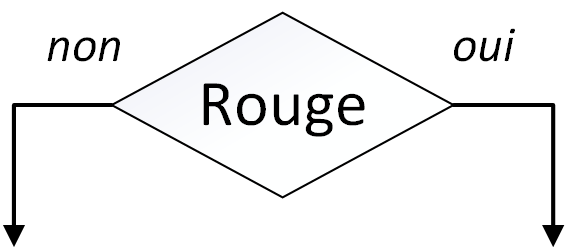
\includegraphics[scale=0.55]{img/DecisionTree_Node_dec.png}
\end{center}

  \end{minipage}
  \hfillx
  \begin{minipage}{0.70\textwidth}
    \centering

% %*   *)
\begin{lstlisting}[language=C,commentstyle=\color{commentgreen}]
struct d_node {
  char *carac;  // Caracteristique : Rouge
  char *etq_fg; // Etiquette Fils Gauche : non
  struct d_node *fg;
  char *etq_fd; // Etiquette Fils Droit  : oui
  struct d_node *fd;
}; \end{lstlisting}

  \end{minipage}
\end{table}

\vspace*{-1.0cm}

\begin{table}[ht!]
  \centering
  \begin{minipage}{0.30\textwidth}
    \centering

\begin{center}

\includegraphics[scale=0.80]{img/DecisionTree_Node_name.png}
\end{center}

  \end{minipage}
  \hfillx
  \begin{minipage}{0.70\textwidth}
    \centering

% %*   *)
\begin{lstlisting}[language=C,commentstyle=\color{commentgreen}]
struct d_node {
  char *carac;       // Caracteristique : Wendy
  char *etq_fg;
  struct d_node *fg; // fg = NULL
  char *etq_fd;
  struct d_node *fd; // fd = NULL
}; \end{lstlisting}

  \end{minipage}
\end{table}

%\bigskip
\vspace*{-0.5cm}

%%%%%%%%%%%%%

\noindent \textbf{Fonctions autorisées}

\medskip

% %*   *)
\begin{lstlisting}[language=C,commentstyle=\color{commentgreen}]
int strlen(char *str);
int strcmp(char *str1, char *str2);
char *get_next_token(char *str, int index);
\end{lstlisting}
%int next_token(char *str, int index);
%char *get_token(char *str, int index);

\vspace*{-0.5cm}

\begin{itemize}
\item \TTBF{strlen(str)} : retourne la longueur de la chaîne \textit{str}
\item \TTBF{strcmp(str1, str2)} : retourne 0 si la chaîne \textit{str1} est égale à la chaîne \textit{str2}
%\item \TTBF{next\_token(str, index)} : retourne l'index de la $1^{\text{ère}}$ lettre du prochain mot dans \textit{str}
%\item \TTBF{get\_token(str, index)} : extrait une sous-chaîne dans \textit{str} à partir de index jusqu'à l'espace suivant ou la fin de chaîne (la sous-chaîne est allouée par malloc dans une adresse à part)
\item \TTBF{get\_next\_token(str, index)} : extrait une sous-chaîne dans \textit{str} à partir de \textit{index} jusqu'à l'espace suivant ou jusqu'à la fin de chaîne (la sous-chaîne est allouée dans un espace mémoire à part avec malloc). Lorsque la fonction atteint un \TTBF{'\textbackslash 0'} ou que \textit{str} est \TTBF{NULL}, elle renvoie \TTBF{NULL}.
\end{itemize}

%%%%%%%%%%%%%

\begin{center}
%\GrilleReponseN{13}
\GrilleReponseTextUp{17.5}{0}{\TTBF{\textcolor{blue}{char} *get\_friend(\textcolor{blue}{d\_node} *root, \textcolor{blue}{char} *str)}}
\end{center}

%\medskip

%%%%%%%%%%%%%%%%%%%%%%%%%%%%%%%%

\subsection{(0 point) That's all Folks!}

\noindent Félicitations, vous avez atteint la fin du partiel et terminé l'année !
Vérifiez bien d'avoir écrit vos nom et prénom sur la première page, et s'il vous reste du temps... n'hésitez pas à dessiner un Cartman ou un Kenny ornithorynque ou autre chose (tant que cela reste correct et n'entraînera donc aucun EpiSignalement).

\begin{center}

{\small \textit{(cette image non plus n'est pas de moi)} }

\medskip


\includegraphics[scale=0.2]{img/kenny-mccormick_platypus.png}

\end{center}

\clearpage

%%%%%%%%%%%%%%%%%%%%%%%%%%%%%%%%%%%%%%%%%%%%%%%%%%%%%%%%

%\thispagestyle{empty}

\vfillFirst

\begin{center}

\begin{LARGE}
\textbf{CORRECTION SUJET A}

\bigskip

\textbf{\MakeUppercase{\TitreMatiere}}
\end{LARGE}

\end{center}

\vfillLast

\end{document}
